\documentclass[12pt, a4paper]{article}
\usepackage[margin=0.5in]{geometry}

\usepackage{color}
\usepackage[dvipsnames]{xcolor}
\usepackage{hyperref}
\hypersetup{
    colorlinks=true,
    linkcolor=blue,
    urlcolor=blue,
    linktoc=all
}


\usepackage{amsmath}
\usepackage{mathtools}
\usepackage{amssymb}
\usepackage{cancel}
\usepackage{bm}
\usepackage{dsfont}
\usepackage{graphicx}
\usepackage{graphics}
\usepackage{xfrac}
\usepackage{array}
\setcounter{MaxMatrixCols}{40}

\usepackage{ulem} %just so I can strike through items on my todo list using \sout{text to be struck through}

\usepackage{enumerate}
\usepackage{enumitem}
\usepackage{multirow}

%inclusions carried over from past class homework formats
\usepackage{units}
\usepackage{fullpage}
\usepackage{alltt}
\usepackage{mathrsfs}
\usepackage{xcolor}
\usepackage{soul}

\usepackage{pgfplots}

\DeclarePairedDelimiter{\abs}{\lvert}{\rvert}
\newcommand*{\fontCourier}{\fontfamily{pcr}\selectfont}
\newcommand*\mean[1]{\overline{#1}}
\newcommand\scalemath[2]{\scalebox{#1}{\mbox{\ensuremath{\displaystyle #2}}}}

\setcounter{tocdepth}{5}
\setcounter{secnumdepth}{5}

% \usepackage{pdfpages}
\usepackage{Sweave}
\begin{document}
% 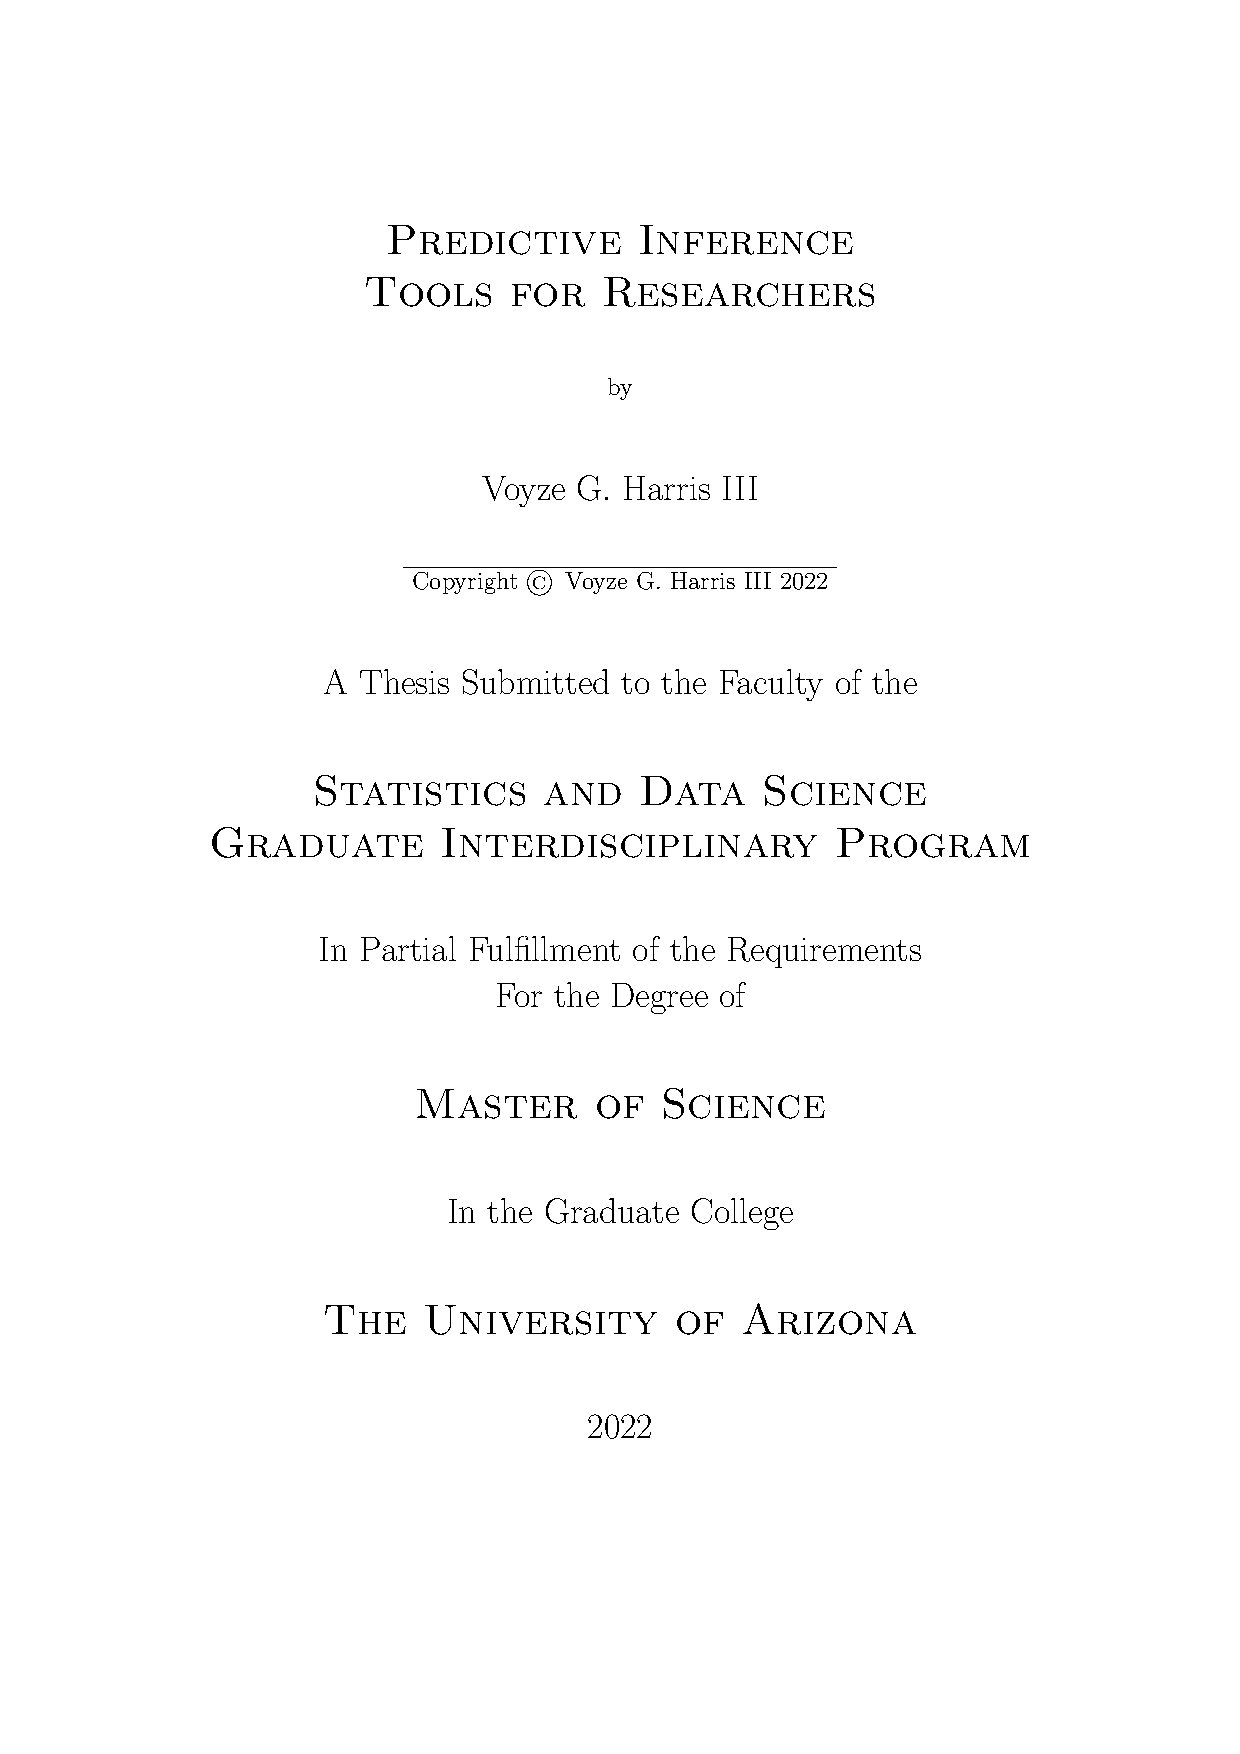
\includepdf{TitlePage_MastersThesis}
% 
\includepdf{ThesisApprovalPage}
\Sconcordance{concordance:ToDoList.tex:ToDoList.Rnw:%
1 51 1 1 0 7 1 1 4 36 1}


% \tableofcontents
% \newpage



\title{To Do List}
\author{\Large Gabe Harris}
\maketitle

\begin{itemize}
  \item Read intros to listed texts (See Thesis section 2.1 Why Predictive Inference?) and summarize answers to that question in WhyPredictiveInference.Rnw
    \begin{itemize}
      \item Nate Silver's book (1st chapter or intro)
      \item \sout{Hoff's book}
      \item Geyser's book (1st chapter or intro)
      \item Aitchison and Dunsmore (1st chapter or intro)
      \item \sout{Dean's paper}
      \item maybe some googling
    \end{itemize}
  \item \sout{Create example comparing predictive inference result with plug in parameter result}
    \subitem \sout{Dean's suggestion:  1-sample binomial with small sample size.  E.g. 3 successes, 7 failures (Pr(success) < 0.5).  Difference will be more pronounced with smaller sample sizes.}
  \item \textcolor{red}{(1)} Combine rpredNormIG(), rpredNormIG2(), and rpredNormIGk() into one function
  \item Read up on convergence in probability and justification for MCMC (Hoff, Casella \& Berger)
  \item Compare variance computations: var() function on MCMC sample vs direct computation from theory ($EX^2 - (EX)^2$)
  \item \textcolor{red}{(2)}  General guidance:  Read up on ``How to write a thesis in Latex," for example \url{https://www.overleaf.com/learn/latex/How_to_Write_a_Thesis_in_LaTeX_(Part_1)%3A_Basic_Structure}
  \item \textcolor{red}{(3)} Figure formatting:  save figures as .png files and insert?  Or what?  Need better control over how figure appears in resulting pdf.
  \item \textcolor{red}{(0)} Incorporate any guidance from Dean.
  \item Write up explanation of how each function works
\end{itemize}

\begin{itemize}
  \item Exponential-Gamma random sampler:  draw a single theta from posterior or draw a new one for each prediction?  (Can't tell the difference from histograms)
  \item Beta-Binomial:  Use posterior of theta (which is a gamma) and then make prediction based on draw(s) of theta (like I'm doing for Exponential-Gamma?)  Why did I go to the trouble of using the inverse transform method before?
\end{itemize}


{\huge Dean's Notes 1/4/2022}
\begin{enumerate}
  \item \sout{Remove the ``Chapter 1” and “Chapter 2” from the chapter titles.}
  \item \textcolor{red}{question sent back to Dean 1/5}\\
    p 4, Abstract - You know that Bayesian inference need not be predictive.
  \item p 4, section 2.1 \\
    I think you may need a citation for that first  sentence.\\
    I feel like you need several citation in this first paragraph.\\
    How many of these assertions are your original ideas, and how many are borrowed?\\

  \item \textcolor{red}{sent update to Dean 1/5/2022} p 5  What are the take-aways from this example?
  \item p 8 Ch3  intro paragraph\\
    Yes - add an intro paragraph\\
    What about these problems makes them unique? or simple?\\
    Also, describe (list) the problems you are going to address.\\
  \item p9, bottom - The random sampling should work the same either way.  \textcolor{red}{Is one method preferable?}
  \item p10, bottom \\
    The likelihood is a function of the parameter conditional on the data.\\\\

\textcolor{blue}{Ok is the point that we're talking about a posterior distribution of $\theta$?  This is the only place in the paper that I talk in terms of Likelihood, and the only reason I do it is that Geisser made the switch here.}\\\\

    The conventional use of upper and lower case values for variables you know that Y is unobserved, y is observed.\\\\

    Switching to the likelihood notation is a little less cumbersome.  \\
    For discrete PMFs (like the binomial), the expression would be\\
    Pr$(Y1 = y1,...,Yn=yn | \theta)$\\\\

    For continuous pdfs its trickier.\\\\

    You can use whichever notation you like - but you have to define it if it’s unusual.  It needs to be clear what you are conditioning on, and what is unknown (or random)\\\\
    \textcolor{blue}{By ``whichever notation" do you mean choosing between $p(\theta|data)$ and $L(\theta)$?  Also, if I go with likelihood, do I need to say $L(\theta|data)$ or is there no need because ``given the data" is understood by definition of likelihood?}
  \item \sout{p 11 - first para.  For the sentences above, I presume you want some censoring value and not a parameter theta?}
  \item p17 - section 3.3.3  I also don't know where you got this example. \textcolor{blue}{Discuss over Zoom}
  \item p21 3.4.1.3 - I don't think you need other values for kappa or nu.
  \item p24. 3.4.2.3 - I would probably just say that Hoff provides the following example and we reproduce his description.
  \item p27. The two-column format would be more standard, and would fit better with the “tidy” data format.  It would be easier to use.
  \item p 33.  ``Comparing the values of ߈ols to their standard errors:”\\
    This is the usual regression t-statistic for regression parameter estimates.
  \item This is as far as I got.\\
    dean

\end{enumerate}











\end{document}
